\documentclass{article}
\usepackage{enumitem}
\usepackage{amsmath}
\usepackage{tikz}
\usepackage{array}
\usepackage{graphicx}
\usepackage[utf8]{inputenc}   % Suporte para codificação UTF-8
\usetikzlibrary{positioning}
\usetikzlibrary{graphs}

\renewcommand\thesubsection{\arabic{subsection}} % Hace que subsección use solo números (1, 2, 3, etc.)
\setcounter{secnumdepth}{2} % Asegura que las subsecciones se numerarán

\title{AULA11: Exercício teórico Grafos busca largura e profundidade}
\author{Aluno: Gian Franco Joel Condori Luna}
\date{\today}

\begin{document}

\maketitle

\section*{Exercices}
\setcounter{section}{1}
\subsection {(0.4) Considere o grafo abaixo:}
  \begin{enumerate}[label=\alph*)]
    \item Mostre como a busca em profundidade funciona nele, iniciando no vértice q.
    \item Mostre como a busca em largura funciona nele, iniciando no vértice q.
    \item Um ciclo corresponde a um caminho no grafo saindo e retornando ao mesmo
    ponto. Indique quais vértices formam ciclo no grafo.
    \item Indique quais arestas devo remover no grafo para formar três componentes.
  \end{enumerate}
  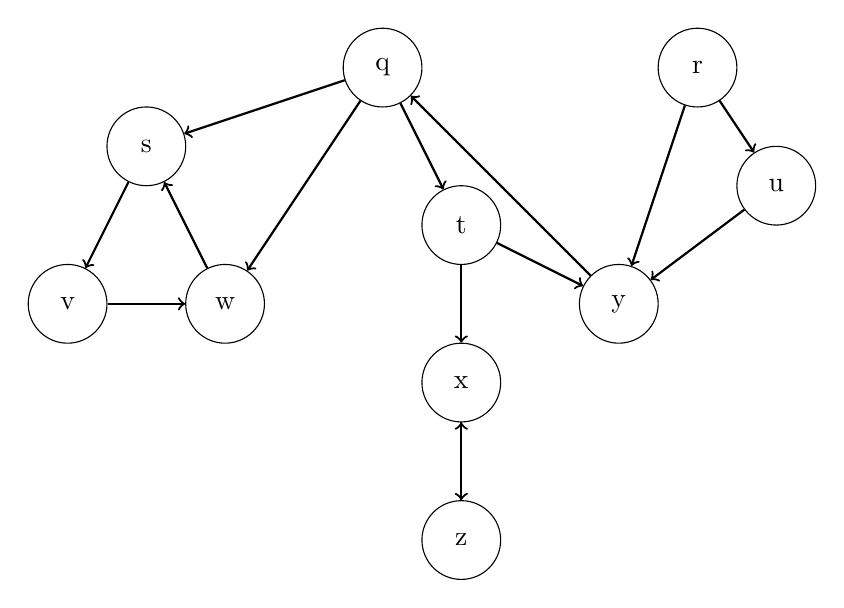
\begin{tikzpicture}[every node/.style={draw, circle, minimum size=1cm}]
    % Nodos
    \node (v) at (0,0) {v};
    \node (s) at (1,2) {s};
    \node (w) at (2,0) {w};
    \node (q) at (4,3) {q};
    \node (t) at (5,1) {t};
    \node (y) at (7,0) {y};
    \node (r) at (8,3) {r};
    \node (u) at (9,1.5) {u};
    \node (x) at (5,-1) {x};
    \node (z) at (5,-3) {z};
    
    % Aristas
    \draw[->, thick] (s) -- (v);
    \draw[->, thick] (v) -- (w);
    \draw[->, thick] (w) -- (s);
    \draw[->, thick] (q) -- (s);
    \draw[->, thick] (q) -- (w);
    \draw[->, thick] (q) -- (t);
    \draw[->, thick] (t) -- (y);
    \draw[->, thick] (y) -- (q);
    \draw[->, thick] (r) -- (y);
    \draw[->, thick] (u) -- (y);
    \draw[->, thick] (r) -- (u);
    \draw[->, thick] (t) -- (x);
    \draw[->, thick] (x) -- (z);
    \draw[->, thick] (z) -- (x);
  \end{tikzpicture}
  
\subsubsection{Solução:}
  \begin{enumerate}[label=\alph*)]
    \item Busca em profundidade iniciando vértice q
      \begin{enumerate}[label=\textbullet]
        \item Passo 1: O nó inicio é o nó "q" e é adicionado na pilha
        \begin{center}
          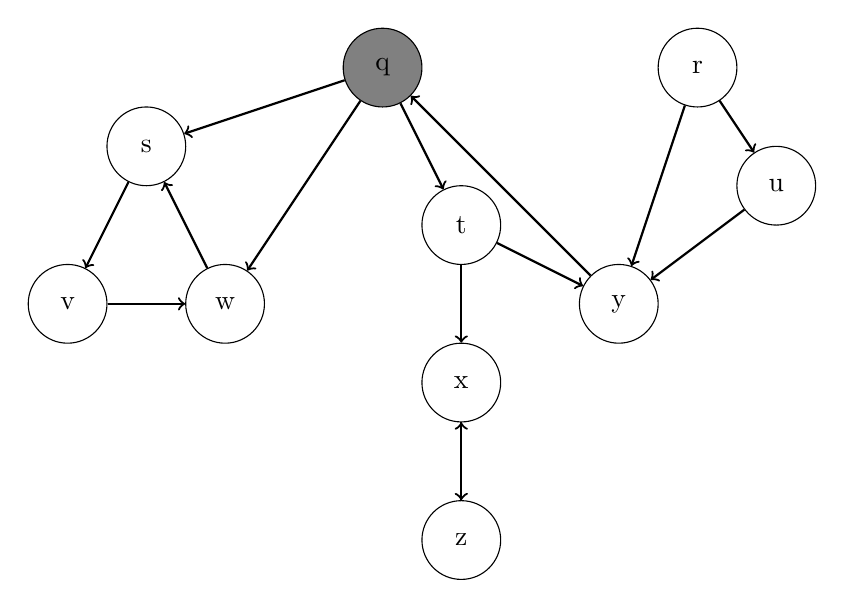
\begin{tikzpicture}[every node/.style={draw, circle, minimum size=1cm}]
            % Nodos
            \node (v) at (0,0) {v};
            \node (s) at (1,2) {s};
            \node (w) at (2,0) {w};
            \node[draw, circle, fill=gray] (q) at (4,3) {q};
            \node (t) at (5,1) {t};
            \node (y) at (7,0) {y};
            \node (r) at (8,3) {r};
            \node (u) at (9,1.5) {u};
            \node (x) at (5,-1) {x};
            \node (z) at (5,-3) {z};
            
            % Aristas
            \draw[->, thick] (s) -- (v);
            \draw[->, thick] (v) -- (w);
            \draw[->, thick] (w) -- (s);
            \draw[->, thick] (q) -- (s);
            \draw[->, thick] (q) -- (w);
            \draw[->, thick] (q) -- (t);
            \draw[->, thick] (t) -- (y);
            \draw[->, thick] (y) -- (q);
            \draw[->, thick] (r) -- (y);
            \draw[->, thick] (u) -- (y);
            \draw[->, thick] (r) -- (u);
            \draw[->, thick] (t) -- (x);
            \draw[->, thick] (x) -- (z);
            \draw[->, thick] (z) -- (x);
          \end{tikzpicture}
        \end{center}
        \[
          \scalebox{1.5}{$
            \begin{array}{|c|}
                \hline
                q \\ 
                \hline
            \end{array}
          $}
        \]

        
        \item Passo 2: O nó "q" tem nó adjacente "s" e esse é adicionado na pilha.
        \begin{center}
          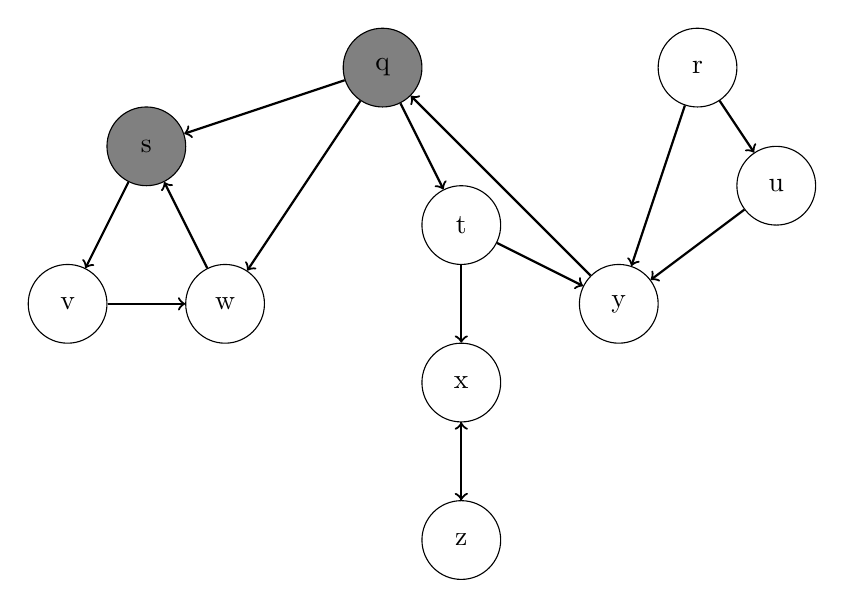
\begin{tikzpicture}[every node/.style={draw, circle, minimum size=1cm}]
            % Nodos
            \node (v) at (0,0) {v};
            \node[draw, circle, fill=gray] (s) at (1,2) {s};
            \node (w) at (2,0) {w};
            \node[draw, circle, fill=gray] (q) at (4,3) {q};
            \node (t) at (5,1) {t};
            \node (y) at (7,0) {y};
            \node (r) at (8,3) {r};
            \node (u) at (9,1.5) {u};
            \node (x) at (5,-1) {x};
            \node (z) at (5,-3) {z};
            
            % Aristas
            \draw[->, thick] (s) -- (v);
            \draw[->, thick] (v) -- (w);
            \draw[->, thick] (w) -- (s);
            \draw[->, thick] (q) -- (s);
            \draw[->, thick] (q) -- (w);
            \draw[->, thick] (q) -- (t);
            \draw[->, thick] (t) -- (y);
            \draw[->, thick] (y) -- (q);
            \draw[->, thick] (r) -- (y);
            \draw[->, thick] (u) -- (y);
            \draw[->, thick] (r) -- (u);
            \draw[->, thick] (t) -- (x);
            \draw[->, thick] (x) -- (z);
            \draw[->, thick] (z) -- (x);
          \end{tikzpicture}
        \end{center}
        \[
          \scalebox{1.5}{$
            \begin{array}{|c|}
                \hline
                s \\ 
                \hline
                q \\ 
                \hline
            \end{array}
          $}
        \]

        \item Passo 3: O nó "s" tem nó adjacente "v" e esse é adicionado na pilha.
        \begin{center}
          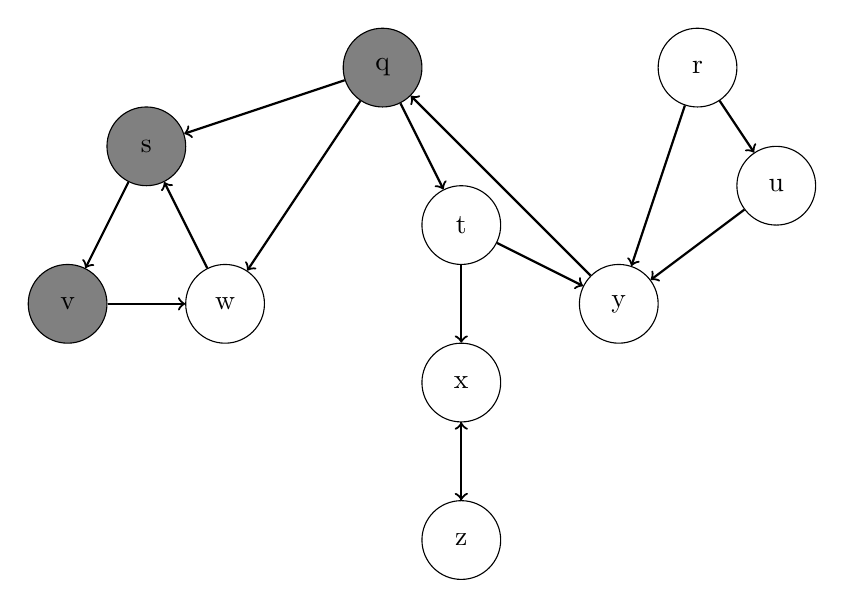
\begin{tikzpicture}[every node/.style={draw, circle, minimum size=1cm}]
            % Nodos
            \node[draw, circle, fill=gray] (v) at (0,0) {v};
            \node[draw, circle, fill=gray] (s) at (1,2) {s};
            \node (w) at (2,0) {w};
            \node[draw, circle, fill=gray] (q) at (4,3) {q};
            \node (t) at (5,1) {t};
            \node (y) at (7,0) {y};
            \node (r) at (8,3) {r};
            \node (u) at (9,1.5) {u};
            \node (x) at (5,-1) {x};
            \node (z) at (5,-3) {z};
            
            % Aristas
            \draw[->, thick] (s) -- (v);
            \draw[->, thick] (v) -- (w);
            \draw[->, thick] (w) -- (s);
            \draw[->, thick] (q) -- (s);
            \draw[->, thick] (q) -- (w);
            \draw[->, thick] (q) -- (t);
            \draw[->, thick] (t) -- (y);
            \draw[->, thick] (y) -- (q);
            \draw[->, thick] (r) -- (y);
            \draw[->, thick] (u) -- (y);
            \draw[->, thick] (r) -- (u);
            \draw[->, thick] (t) -- (x);
            \draw[->, thick] (x) -- (z);
            \draw[->, thick] (z) -- (x);
          \end{tikzpicture}
        \end{center}
        \[
          \scalebox{1.5}{$
            \begin{array}{|c|}
                \hline
                v \\ 
                \hline
                s \\ 
                \hline
                q \\ 
                \hline
            \end{array}
          $}
        \]

        \item Passo 4: O nó "v" tem nó adjacente "w" e esse é adicionado na pilha.
        \begin{center}
          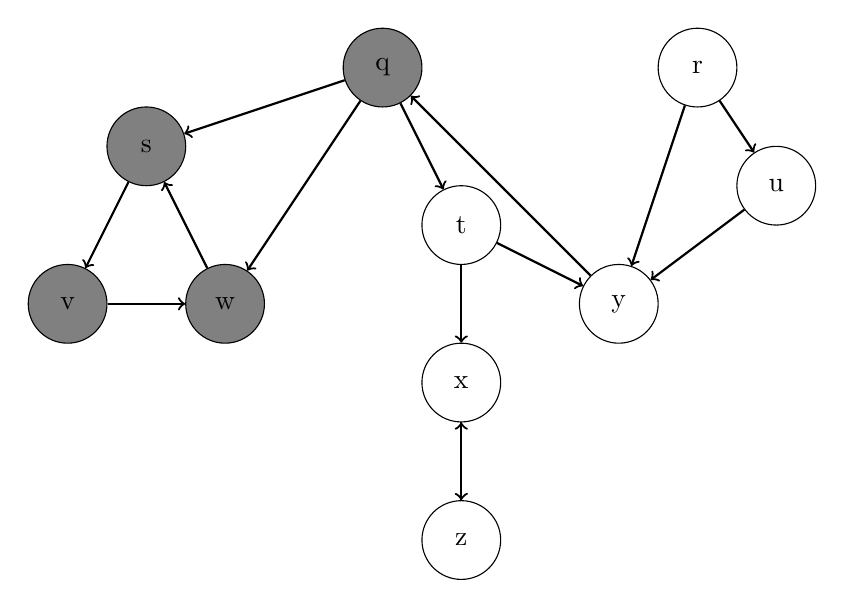
\begin{tikzpicture}[every node/.style={draw, circle, minimum size=1cm}]
            % Nodos
            \node[draw, circle, fill=gray] (v) at (0,0) {v};
            \node[draw, circle, fill=gray] (s) at (1,2) {s};
            \node[draw, circle, fill=gray] (w) at (2,0) {w};
            \node[draw, circle, fill=gray] (q) at (4,3) {q};
            \node (t) at (5,1) {t};
            \node (y) at (7,0) {y};
            \node (r) at (8,3) {r};
            \node (u) at (9,1.5) {u};
            \node (x) at (5,-1) {x};
            \node (z) at (5,-3) {z};
            
            % Aristas
            \draw[->, thick] (s) -- (v);
            \draw[->, thick] (v) -- (w);
            \draw[->, thick] (w) -- (s);
            \draw[->, thick] (q) -- (s);
            \draw[->, thick] (q) -- (w);
            \draw[->, thick] (q) -- (t);
            \draw[->, thick] (t) -- (y);
            \draw[->, thick] (y) -- (q);
            \draw[->, thick] (r) -- (y);
            \draw[->, thick] (u) -- (y);
            \draw[->, thick] (r) -- (u);
            \draw[->, thick] (t) -- (x);
            \draw[->, thick] (x) -- (z);
            \draw[->, thick] (z) -- (x);
          \end{tikzpicture}
        \end{center}
        \[
          \scalebox{1.5}{$
            \begin{array}{|c|}
                \hline
                w \\ 
                \hline
                v \\ 
                \hline
                s \\ 
                \hline
                q \\ 
                \hline
            \end{array}
          $}
        \]

        \item Passo 5: Removo nó "w" da pilha porque não tem mais nós adjacentes
        \begin{center}
          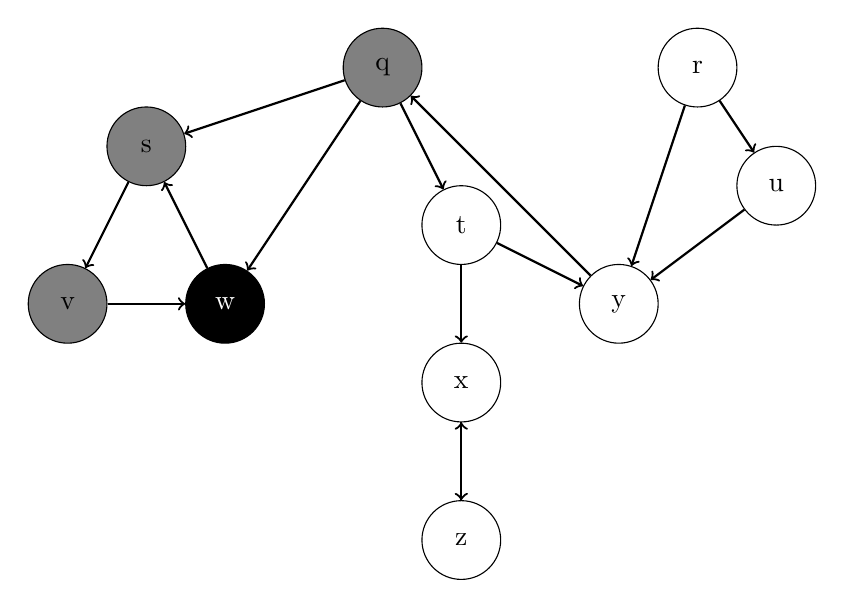
\begin{tikzpicture}[every node/.style={draw, circle, minimum size=1cm}]
            % Nodos
            \node[draw, circle, fill=gray] (v) at (0,0) {v};
            \node[draw, circle, fill=gray] (s) at (1,2) {s};
            \node[draw, circle, fill=black, text=white] (w) at (2,0) {w};
            \node[draw, circle, fill=gray] (q) at (4,3) {q};
            \node (t) at (5,1) {t};
            \node (y) at (7,0) {y};
            \node (r) at (8,3) {r};
            \node (u) at (9,1.5) {u};
            \node (x) at (5,-1) {x};
            \node (z) at (5,-3) {z};
            
            % Aristas
            \draw[->, thick] (s) -- (v);
            \draw[->, thick] (v) -- (w);
            \draw[->, thick] (w) -- (s);
            \draw[->, thick] (q) -- (s);
            \draw[->, thick] (q) -- (w);
            \draw[->, thick] (q) -- (t);
            \draw[->, thick] (t) -- (y);
            \draw[->, thick] (y) -- (q);
            \draw[->, thick] (r) -- (y);
            \draw[->, thick] (u) -- (y);
            \draw[->, thick] (r) -- (u);
            \draw[->, thick] (t) -- (x);
            \draw[->, thick] (x) -- (z);
            \draw[->, thick] (z) -- (x);
          \end{tikzpicture}
        \end{center}
        \[
          \scalebox{1.5}{$
            \begin{array}{|c|} 
                \hline
                v \\ 
                \hline
                s \\ 
                \hline
                q \\ 
                \hline
            \end{array}
          $}
        \]

        \item Passo 6: Removo nó "v" da pilha porque não tem mais nós adjacentes
        \begin{center}
          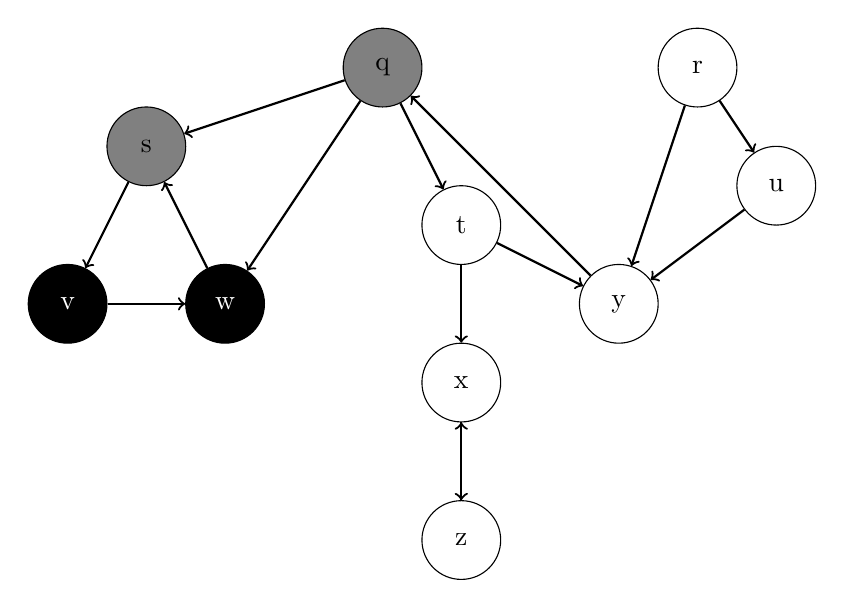
\begin{tikzpicture}[every node/.style={draw, circle, minimum size=1cm}]
            % Nodos
            \node[draw, circle, fill=black, text=white] (v) at (0,0) {v};
            \node[draw, circle, fill=gray] (s) at (1,2) {s};
            \node[draw, circle, fill=black, text=white] (w) at (2,0) {w};
            \node[draw, circle, fill=gray] (q) at (4,3) {q};
            \node (t) at (5,1) {t};
            \node (y) at (7,0) {y};
            \node (r) at (8,3) {r};
            \node (u) at (9,1.5) {u};
            \node (x) at (5,-1) {x};
            \node (z) at (5,-3) {z};
            
            % Aristas
            \draw[->, thick] (s) -- (v);
            \draw[->, thick] (v) -- (w);
            \draw[->, thick] (w) -- (s);
            \draw[->, thick] (q) -- (s);
            \draw[->, thick] (q) -- (w);
            \draw[->, thick] (q) -- (t);
            \draw[->, thick] (t) -- (y);
            \draw[->, thick] (y) -- (q);
            \draw[->, thick] (r) -- (y);
            \draw[->, thick] (u) -- (y);
            \draw[->, thick] (r) -- (u);
            \draw[->, thick] (t) -- (x);
            \draw[->, thick] (x) -- (z);
            \draw[->, thick] (z) -- (x);
          \end{tikzpicture}
        \end{center}
        \[
          \scalebox{1.5}{$
            \begin{array}{|c|} 
                \hline
                s \\ 
                \hline
                q \\ 
                \hline
            \end{array}
          $}
        \]

        \item Passo 7: Removo nó "s" da pilha porque não tem mais nós adjacentes
        \begin{center}
          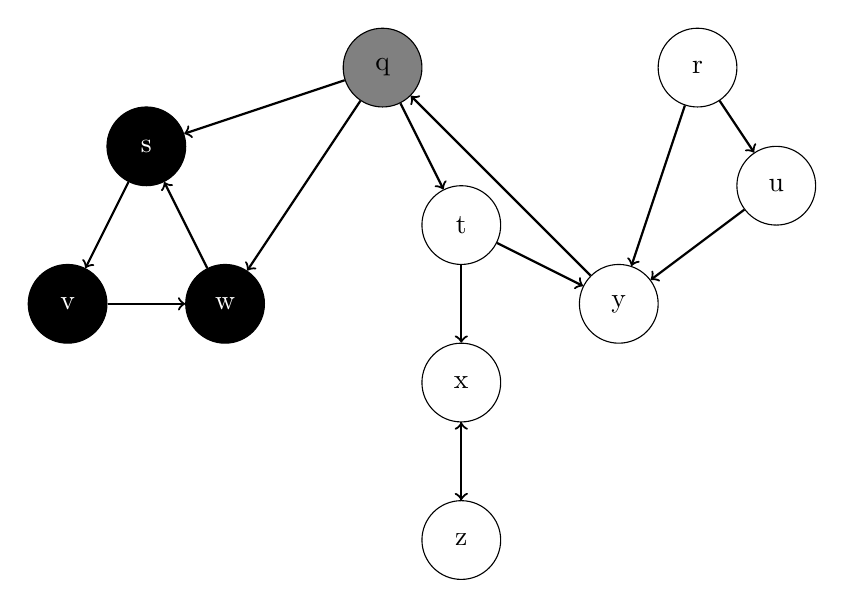
\begin{tikzpicture}[every node/.style={draw, circle, minimum size=1cm}]
            % Nodos
            \node[draw, circle, fill=black, text=white] (v) at (0,0) {v};
            \node[draw, circle, fill=black, text=white] (s) at (1,2) {s};
            \node[draw, circle, fill=black, text=white] (w) at (2,0) {w};
            \node[draw, circle, fill=gray] (q) at (4,3) {q};
            \node (t) at (5,1) {t};
            \node (y) at (7,0) {y};
            \node (r) at (8,3) {r};
            \node (u) at (9,1.5) {u};
            \node (x) at (5,-1) {x};
            \node (z) at (5,-3) {z};
            
            % Aristas
            \draw[->, thick] (s) -- (v);
            \draw[->, thick] (v) -- (w);
            \draw[->, thick] (w) -- (s);
            \draw[->, thick] (q) -- (s);
            \draw[->, thick] (q) -- (w);
            \draw[->, thick] (q) -- (t);
            \draw[->, thick] (t) -- (y);
            \draw[->, thick] (y) -- (q);
            \draw[->, thick] (r) -- (y);
            \draw[->, thick] (u) -- (y);
            \draw[->, thick] (r) -- (u);
            \draw[->, thick] (t) -- (x);
            \draw[->, thick] (x) -- (z);
            \draw[->, thick] (z) -- (x);
          \end{tikzpicture}
        \end{center}
        \[
          \scalebox{1.5}{$
            \begin{array}{|c|} 
                \hline
                q \\ 
                \hline
            \end{array}
          $}
        \]

        \item Passo 8: O nó "q" tem nó adjacente "t" e esse é adicionado na pilha.
        \begin{center}
          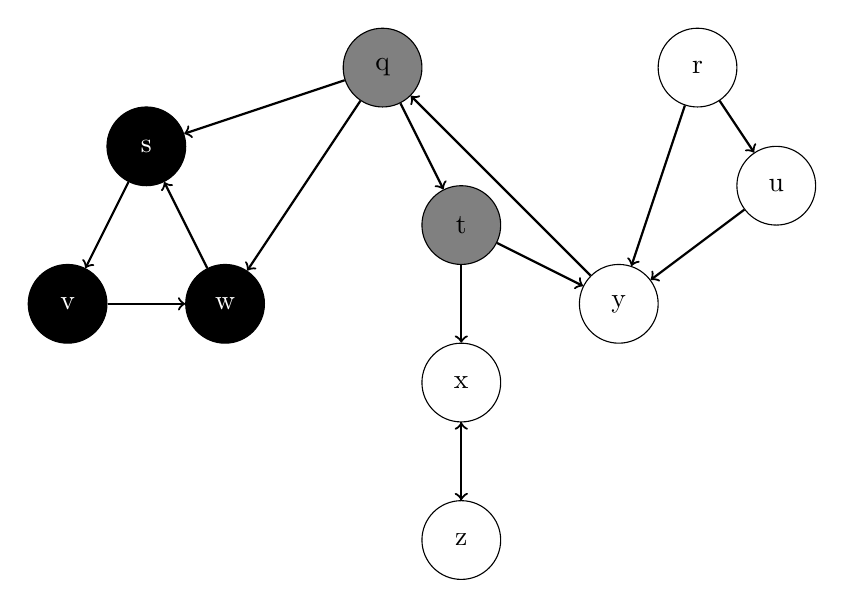
\begin{tikzpicture}[every node/.style={draw, circle, minimum size=1cm}]
            % Nodos
            \node[draw, circle, fill=black, text=white] (v) at (0,0) {v};
            \node[draw, circle, fill=black, text=white] (s) at (1,2) {s};
            \node[draw, circle, fill=black, text=white] (w) at (2,0) {w};
            \node[draw, circle, fill=gray] (q) at (4,3) {q};
            \node[draw, circle, fill=gray] (t) at (5,1) {t};
            \node (y) at (7,0) {y};
            \node (r) at (8,3) {r};
            \node (u) at (9,1.5) {u};
            \node (x) at (5,-1) {x};
            \node (z) at (5,-3) {z};
            
            % Aristas
            \draw[->, thick] (s) -- (v);
            \draw[->, thick] (v) -- (w);
            \draw[->, thick] (w) -- (s);
            \draw[->, thick] (q) -- (s);
            \draw[->, thick] (q) -- (w);
            \draw[->, thick] (q) -- (t);
            \draw[->, thick] (t) -- (y);
            \draw[->, thick] (y) -- (q);
            \draw[->, thick] (r) -- (y);
            \draw[->, thick] (u) -- (y);
            \draw[->, thick] (r) -- (u);
            \draw[->, thick] (t) -- (x);
            \draw[->, thick] (x) -- (z);
            \draw[->, thick] (z) -- (x);
          \end{tikzpicture}
        \end{center}
        \[
          \scalebox{1.5}{$
            \begin{array}{|c|} 
                \hline
                t \\ 
                \hline
                q \\ 
                \hline
            \end{array}
          $}
        \]


        \item Passo 9: O nó "t" tem nó adjacente "x" e esse é adicionado na pilha.
        \begin{center}
          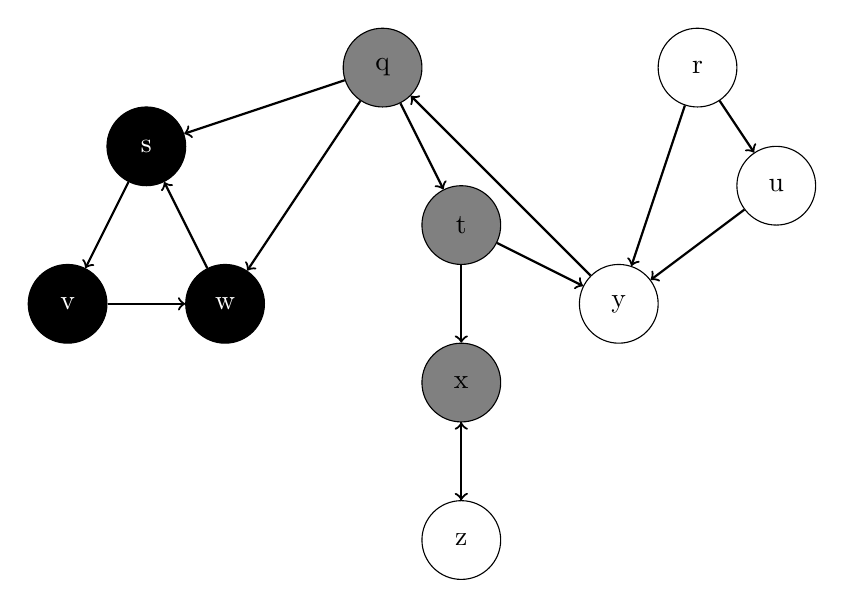
\begin{tikzpicture}[every node/.style={draw, circle, minimum size=1cm}]
            % Nodos
            \node[draw, circle, fill=black, text=white] (v) at (0,0) {v};
            \node[draw, circle, fill=black, text=white] (s) at (1,2) {s};
            \node[draw, circle, fill=black, text=white] (w) at (2,0) {w};
            \node[draw, circle, fill=gray] (q) at (4,3) {q};
            \node[draw, circle, fill=gray] (t) at (5,1) {t};
            \node (y) at (7,0) {y};
            \node (r) at (8,3) {r};
            \node (u) at (9,1.5) {u};
            \node[draw, circle, fill=gray] (x) at (5,-1) {x};
            \node (z) at (5,-3) {z};
            
            % Aristas
            \draw[->, thick] (s) -- (v);
            \draw[->, thick] (v) -- (w);
            \draw[->, thick] (w) -- (s);
            \draw[->, thick] (q) -- (s);
            \draw[->, thick] (q) -- (w);
            \draw[->, thick] (q) -- (t);
            \draw[->, thick] (t) -- (y);
            \draw[->, thick] (y) -- (q);
            \draw[->, thick] (r) -- (y);
            \draw[->, thick] (u) -- (y);
            \draw[->, thick] (r) -- (u);
            \draw[->, thick] (t) -- (x);
            \draw[->, thick] (x) -- (z);
            \draw[->, thick] (z) -- (x);
          \end{tikzpicture}
        \end{center}
        \[
          \scalebox{1.5}{$
            \begin{array}{|c|} 
              \hline
              x \\   
              \hline
              t \\ 
              \hline
              q \\ 
              \hline
            \end{array}
          $}
        \]


        \item Passo 10: O nó "x" tem nó adjacente "z" e esse é adicionado na pilha.
        \begin{center}
          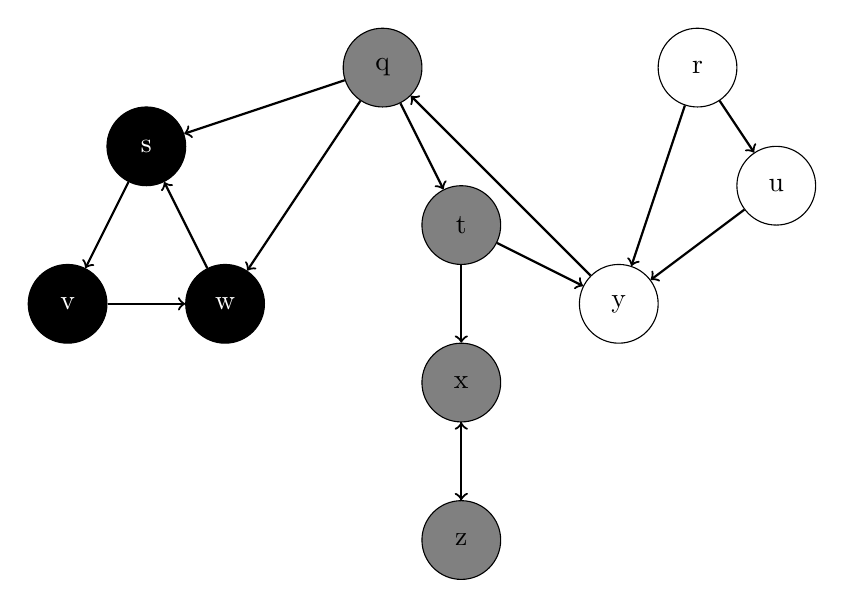
\begin{tikzpicture}[every node/.style={draw, circle, minimum size=1cm}]
            % Nodos
            \node[draw, circle, fill=black, text=white] (v) at (0,0) {v};
            \node[draw, circle, fill=black, text=white] (s) at (1,2) {s};
            \node[draw, circle, fill=black, text=white] (w) at (2,0) {w};
            \node[draw, circle, fill=gray] (q) at (4,3) {q};
            \node[draw, circle, fill=gray] (t) at (5,1) {t};
            \node (y) at (7,0) {y};
            \node (r) at (8,3) {r};
            \node (u) at (9,1.5) {u};
            \node[draw, circle, fill=gray] (x) at (5,-1) {x};
            \node[draw, circle, fill=gray] (z) at (5,-3) {z};
            
            % Aristas
            \draw[->, thick] (s) -- (v);
            \draw[->, thick] (v) -- (w);
            \draw[->, thick] (w) -- (s);
            \draw[->, thick] (q) -- (s);
            \draw[->, thick] (q) -- (w);
            \draw[->, thick] (q) -- (t);
            \draw[->, thick] (t) -- (y);
            \draw[->, thick] (y) -- (q);
            \draw[->, thick] (r) -- (y);
            \draw[->, thick] (u) -- (y);
            \draw[->, thick] (r) -- (u);
            \draw[->, thick] (t) -- (x);
            \draw[->, thick] (x) -- (z);
            \draw[->, thick] (z) -- (x);
          \end{tikzpicture}
        \end{center}
        \[
          \scalebox{1.5}{$
            \begin{array}{|c|}
              \hline
              z \\ 
              \hline
              x \\   
              \hline
              t \\ 
              \hline
              q \\ 
              \hline
            \end{array}
          $}
        \]

        \item Passo 11: Removo nó "z" da pilha porque não tem mais nós adjacentes
        \begin{center}
          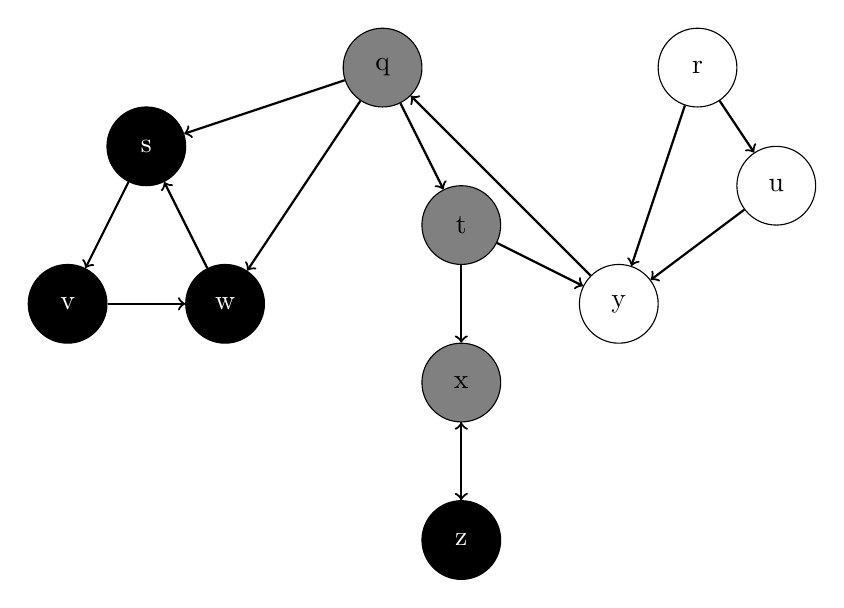
\begin{tikzpicture}[every node/.style={draw, circle, minimum size=1cm}]
            % Nodos
            \node[draw, circle, fill=black, text=white] (v) at (0,0) {v};
            \node[draw, circle, fill=black, text=white] (s) at (1,2) {s};
            \node[draw, circle, fill=black, text=white] (w) at (2,0) {w};
            \node[draw, circle, fill=gray] (q) at (4,3) {q};
            \node[draw, circle, fill=gray] (t) at (5,1) {t};
            \node (y) at (7,0) {y};
            \node (r) at (8,3) {r};
            \node (u) at (9,1.5) {u};
            \node[draw, circle, fill=gray] (x) at (5,-1) {x};
            \node[draw, circle, fill=black, text=white] (z) at (5,-3) {z};
            
            % Aristas
            \draw[->, thick] (s) -- (v);
            \draw[->, thick] (v) -- (w);
            \draw[->, thick] (w) -- (s);
            \draw[->, thick] (q) -- (s);
            \draw[->, thick] (q) -- (w);
            \draw[->, thick] (q) -- (t);
            \draw[->, thick] (t) -- (y);
            \draw[->, thick] (y) -- (q);
            \draw[->, thick] (r) -- (y);
            \draw[->, thick] (u) -- (y);
            \draw[->, thick] (r) -- (u);
            \draw[->, thick] (t) -- (x);
            \draw[->, thick] (x) -- (z);
            \draw[->, thick] (z) -- (x);
          \end{tikzpicture}
        \end{center}
        \[
          \scalebox{1.5}{$
            \begin{array}{|c|}
              \hline
              x \\   
              \hline
              t \\ 
              \hline
              q \\ 
              \hline
            \end{array}
          $}
        \]

        \item Passo 12: Removo nó "x" da pilha porque não tem mais nós adjacentes
        \begin{center}
          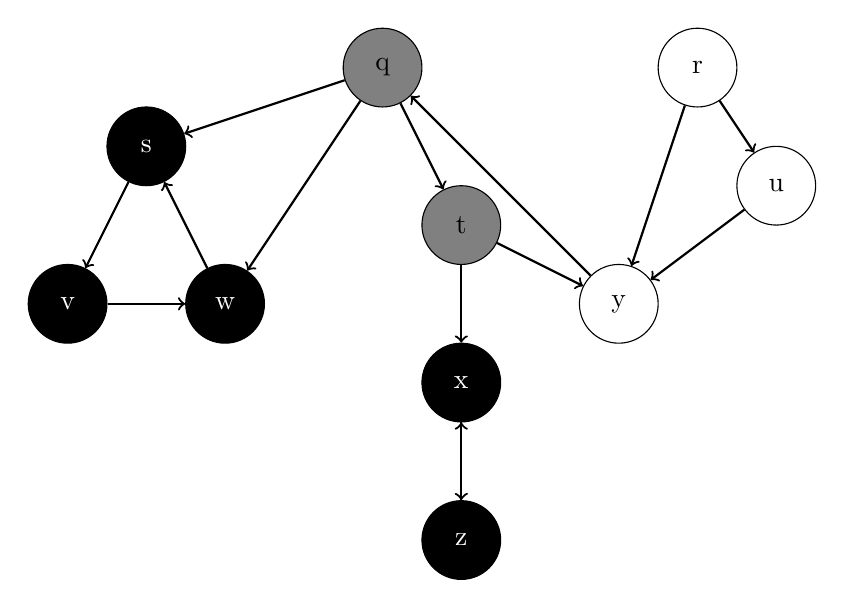
\begin{tikzpicture}[every node/.style={draw, circle, minimum size=1cm}]
            % Nodos
            \node[draw, circle, fill=black, text=white] (v) at (0,0) {v};
            \node[draw, circle, fill=black, text=white] (s) at (1,2) {s};
            \node[draw, circle, fill=black, text=white] (w) at (2,0) {w};
            \node[draw, circle, fill=gray] (q) at (4,3) {q};
            \node[draw, circle, fill=gray] (t) at (5,1) {t};
            \node (y) at (7,0) {y};
            \node (r) at (8,3) {r};
            \node (u) at (9,1.5) {u};
            \node[draw, circle, fill=black, text=white] (x) at (5,-1) {x};
            \node[draw, circle, fill=black, text=white] (z) at (5,-3) {z};
            
            % Aristas
            \draw[->, thick] (s) -- (v);
            \draw[->, thick] (v) -- (w);
            \draw[->, thick] (w) -- (s);
            \draw[->, thick] (q) -- (s);
            \draw[->, thick] (q) -- (w);
            \draw[->, thick] (q) -- (t);
            \draw[->, thick] (t) -- (y);
            \draw[->, thick] (y) -- (q);
            \draw[->, thick] (r) -- (y);
            \draw[->, thick] (u) -- (y);
            \draw[->, thick] (r) -- (u);
            \draw[->, thick] (t) -- (x);
            \draw[->, thick] (x) -- (z);
            \draw[->, thick] (z) -- (x);
          \end{tikzpicture}
        \end{center}
        \[
          \scalebox{1.5}{$
            \begin{array}{|c|}  
              \hline
              t \\ 
              \hline
              q \\ 
              \hline
            \end{array}
          $}
        \]

        \item Passo 13: O nó "t" tem nó adjacente "y" e esse é adicionado na pilha.
        \begin{center}
          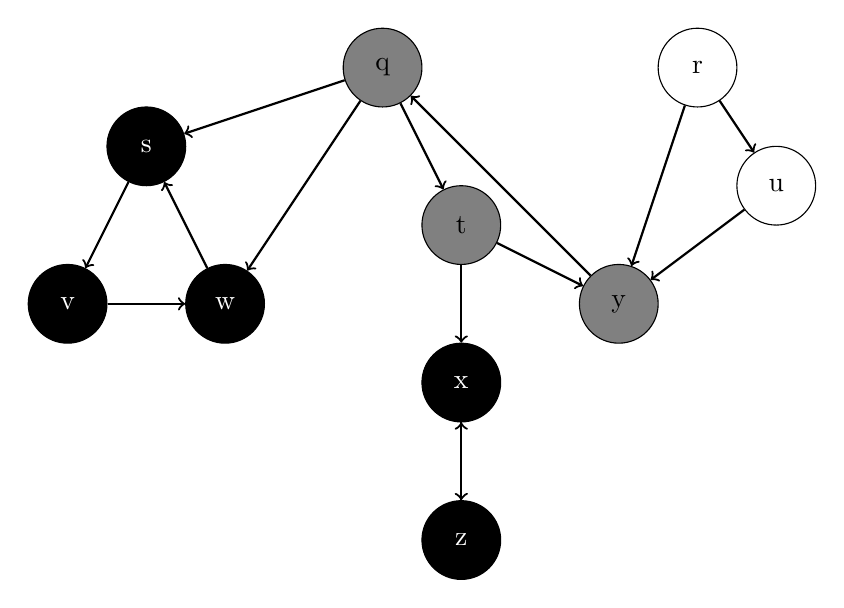
\begin{tikzpicture}[every node/.style={draw, circle, minimum size=1cm}]
            % Nodos
            \node[draw, circle, fill=black, text=white] (v) at (0,0) {v};
            \node[draw, circle, fill=black, text=white] (s) at (1,2) {s};
            \node[draw, circle, fill=black, text=white] (w) at (2,0) {w};
            \node[draw, circle, fill=gray] (q) at (4,3) {q};
            \node[draw, circle, fill=gray] (t) at (5,1) {t};
            \node[draw, circle, fill=gray] (y) at (7,0) {y};
            \node (r) at (8,3) {r};
            \node (u) at (9,1.5) {u};
            \node[draw, circle, fill=black, text=white] (x) at (5,-1) {x};
            \node[draw, circle, fill=black, text=white] (z) at (5,-3) {z};
            
            % Aristas
            \draw[->, thick] (s) -- (v);
            \draw[->, thick] (v) -- (w);
            \draw[->, thick] (w) -- (s);
            \draw[->, thick] (q) -- (s);
            \draw[->, thick] (q) -- (w);
            \draw[->, thick] (q) -- (t);
            \draw[->, thick] (t) -- (y);
            \draw[->, thick] (y) -- (q);
            \draw[->, thick] (r) -- (y);
            \draw[->, thick] (u) -- (y);
            \draw[->, thick] (r) -- (u);
            \draw[->, thick] (t) -- (x);
            \draw[->, thick] (x) -- (z);
            \draw[->, thick] (z) -- (x);
          \end{tikzpicture}
        \end{center}
        \[
          \scalebox{1.5}{$
            \begin{array}{|c|}  
              \hline
              y \\ 
              \hline
              t \\ 
              \hline
              q \\ 
              \hline
            \end{array}
          $}
        \]

        \item Passo 14: Removo nó "y" da pilha porque não tem mais nós adjacentes
        \begin{center}
          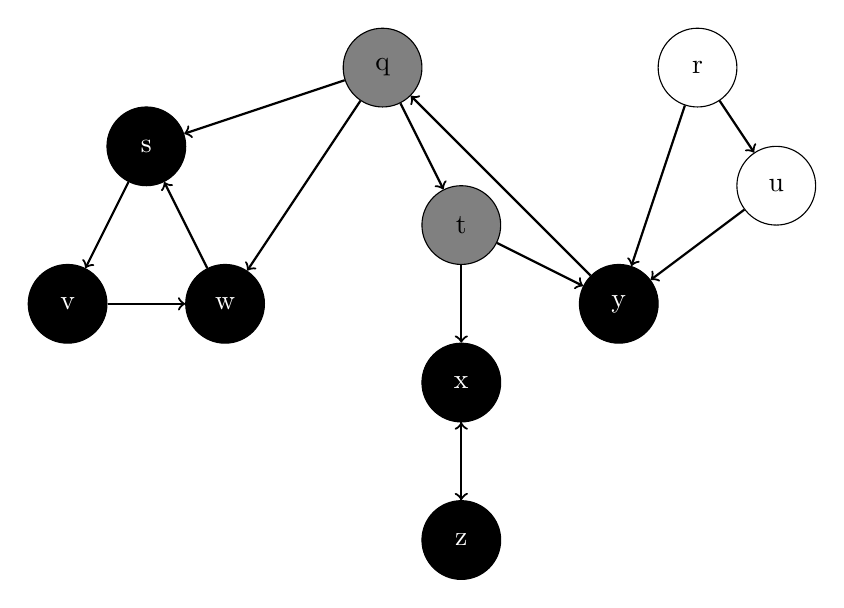
\begin{tikzpicture}[every node/.style={draw, circle, minimum size=1cm}]
            % Nodos
            \node[draw, circle, fill=black, text=white] (v) at (0,0) {v};
            \node[draw, circle, fill=black, text=white] (s) at (1,2) {s};
            \node[draw, circle, fill=black, text=white] (w) at (2,0) {w};
            \node[draw, circle, fill=gray] (q) at (4,3) {q};
            \node[draw, circle, fill=gray] (t) at (5,1) {t};
            \node[draw, circle, fill=black, text=white] (y) at (7,0) {y};
            \node (r) at (8,3) {r};
            \node (u) at (9,1.5) {u};
            \node[draw, circle, fill=black, text=white] (x) at (5,-1) {x};
            \node[draw, circle, fill=black, text=white] (z) at (5,-3) {z};
            
            % Aristas
            \draw[->, thick] (s) -- (v);
            \draw[->, thick] (v) -- (w);
            \draw[->, thick] (w) -- (s);
            \draw[->, thick] (q) -- (s);
            \draw[->, thick] (q) -- (w);
            \draw[->, thick] (q) -- (t);
            \draw[->, thick] (t) -- (y);
            \draw[->, thick] (y) -- (q);
            \draw[->, thick] (r) -- (y);
            \draw[->, thick] (u) -- (y);
            \draw[->, thick] (r) -- (u);
            \draw[->, thick] (t) -- (x);
            \draw[->, thick] (x) -- (z);
            \draw[->, thick] (z) -- (x);
          \end{tikzpicture}
        \end{center}
        \[
          \scalebox{1.5}{$
            \begin{array}{|c|}
              \hline
              t \\ 
              \hline
              q \\ 
              \hline
            \end{array}
          $}
        \]

        \item Passo 15: Removo nó "t" da pilha porque não tem mais nós adjacentes
        \begin{center}
          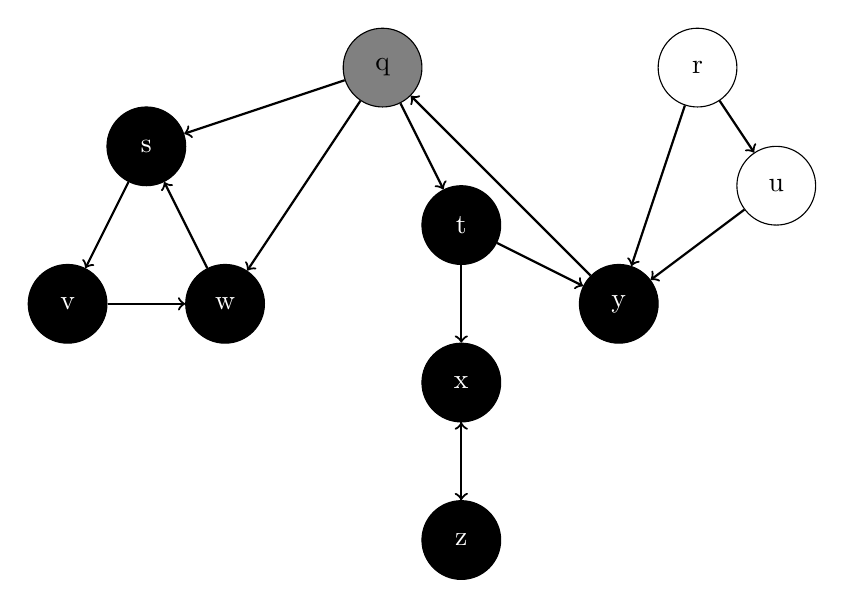
\begin{tikzpicture}[every node/.style={draw, circle, minimum size=1cm}]
            % Nodos
            \node[draw, circle, fill=black, text=white] (v) at (0,0) {v};
            \node[draw, circle, fill=black, text=white] (s) at (1,2) {s};
            \node[draw, circle, fill=black, text=white] (w) at (2,0) {w};
            \node[draw, circle, fill=gray] (q) at (4,3) {q};
            \node[draw, circle, fill=black, text=white] (t) at (5,1) {t};
            \node[draw, circle, fill=black, text=white] (y) at (7,0) {y};
            \node (r) at (8,3) {r};
            \node (u) at (9,1.5) {u};
            \node[draw, circle, fill=black, text=white] (x) at (5,-1) {x};
            \node[draw, circle, fill=black, text=white] (z) at (5,-3) {z};
            
            % Aristas
            \draw[->, thick] (s) -- (v);
            \draw[->, thick] (v) -- (w);
            \draw[->, thick] (w) -- (s);
            \draw[->, thick] (q) -- (s);
            \draw[->, thick] (q) -- (w);
            \draw[->, thick] (q) -- (t);
            \draw[->, thick] (t) -- (y);
            \draw[->, thick] (y) -- (q);
            \draw[->, thick] (r) -- (y);
            \draw[->, thick] (u) -- (y);
            \draw[->, thick] (r) -- (u);
            \draw[->, thick] (t) -- (x);
            \draw[->, thick] (x) -- (z);
            \draw[->, thick] (z) -- (x);
          \end{tikzpicture}
        \end{center}
        \[
          \scalebox{1.5}{$
            \begin{array}{|c|}
              \hline
              q \\ 
              \hline
            \end{array}
          $}
        \]

        \item Passo 16: Removo nó "q" da pilha porque não tem mais nós adjacentes
        \begin{center}
          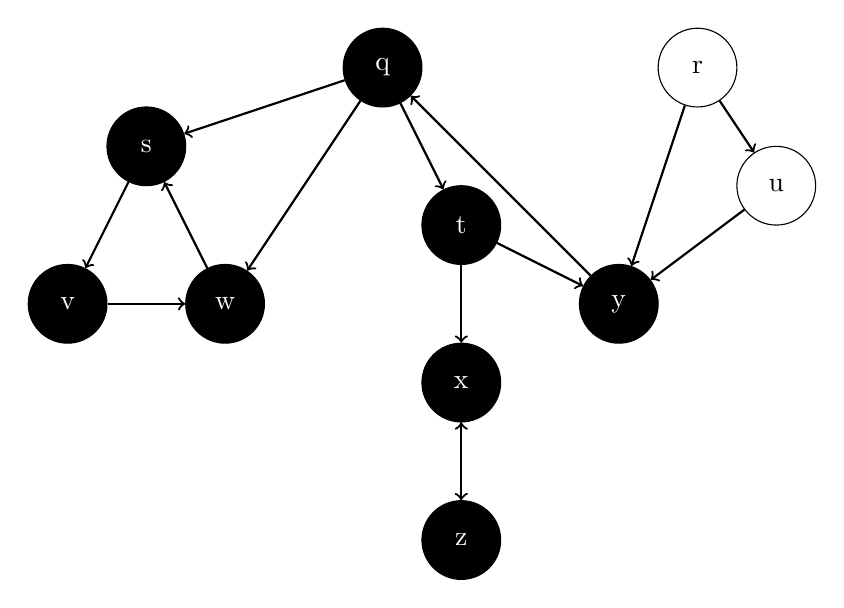
\begin{tikzpicture}[every node/.style={draw, circle, minimum size=1cm}]
            % Nodos
            \node[draw, circle, fill=black, text=white] (v) at (0,0) {v};
            \node[draw, circle, fill=black, text=white] (s) at (1,2) {s};
            \node[draw, circle, fill=black, text=white] (w) at (2,0) {w};
            \node[draw, circle, fill=black, text=white] (q) at (4,3) {q};
            \node[draw, circle, fill=black, text=white] (t) at (5,1) {t};
            \node[draw, circle, fill=black, text=white] (y) at (7,0) {y};
            \node (r) at (8,3) {r};
            \node (u) at (9,1.5) {u};
            \node[draw, circle, fill=black, text=white] (x) at (5,-1) {x};
            \node[draw, circle, fill=black, text=white] (z) at (5,-3) {z};
            
            % Aristas
            \draw[->, thick] (s) -- (v);
            \draw[->, thick] (v) -- (w);
            \draw[->, thick] (w) -- (s);
            \draw[->, thick] (q) -- (s);
            \draw[->, thick] (q) -- (w);
            \draw[->, thick] (q) -- (t);
            \draw[->, thick] (t) -- (y);
            \draw[->, thick] (y) -- (q);
            \draw[->, thick] (r) -- (y);
            \draw[->, thick] (u) -- (y);
            \draw[->, thick] (r) -- (u);
            \draw[->, thick] (t) -- (x);
            \draw[->, thick] (x) -- (z);
            \draw[->, thick] (z) -- (x);
          \end{tikzpicture}
        \end{center}
        \[
          \scalebox{1.5}{$
            \begin{array}{|c|}
              \hline
              \\ 
              \hline
            \end{array}
          $}
        \]

      \end{enumerate}


    \item Busca em largura iniciando vértice q
      \begin{enumerate}[label=\textbullet]
        \item Passo 1: O nó inicio é o nó "q" e é adicionado na filha.
          \begin{center}
            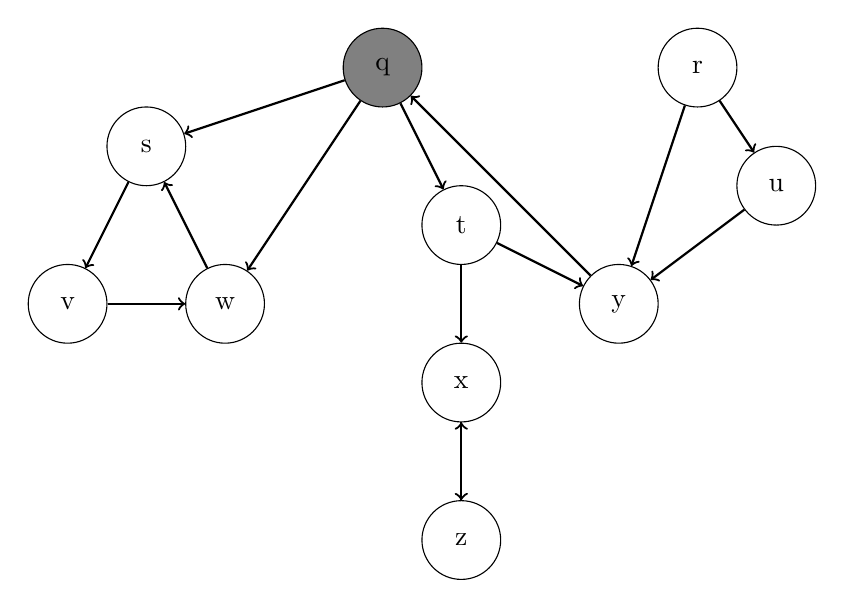
\begin{tikzpicture}[every node/.style={draw, circle, minimum size=1cm}]
              % Nodos
              \node (v) at (0,0) {v};
              \node (s) at (1,2) {s};
              \node (w) at (2,0) {w};
              \node[draw, circle, fill=gray] (q) at (4,3) {q};
              \node (t) at (5,1) {t};
              \node (y) at (7,0) {y};
              \node (r) at (8,3) {r};
              \node (u) at (9,1.5) {u};
              \node (x) at (5,-1) {x};
              \node (z) at (5,-3) {z};
              
              % Aristas
              \draw[->, thick] (s) -- (v);
              \draw[->, thick] (v) -- (w);
              \draw[->, thick] (w) -- (s);
              \draw[->, thick] (q) -- (s);
              \draw[->, thick] (q) -- (w);
              \draw[->, thick] (q) -- (t);
              \draw[->, thick] (t) -- (y);
              \draw[->, thick] (y) -- (q);
              \draw[->, thick] (r) -- (y);
              \draw[->, thick] (u) -- (y);
              \draw[->, thick] (r) -- (u);
              \draw[->, thick] (t) -- (x);
              \draw[->, thick] (x) -- (z);
              \draw[->, thick] (z) -- (x);
            \end{tikzpicture}
          \end{center}
          \[
            \scalebox{1.5}{$
              \begin{array}{|c|c|c|c|c|}
                  \hline
                  q \\ 
                  \hline
              \end{array}
            $}
          \]

        \item Passo 2: Primeiro removo o nó “q” da filha. 
          Em seguida, adiciono seus nós adjacentes à filha; neste caso, os nós adjacentes são "s", "w" e "t".
          \begin{center}
            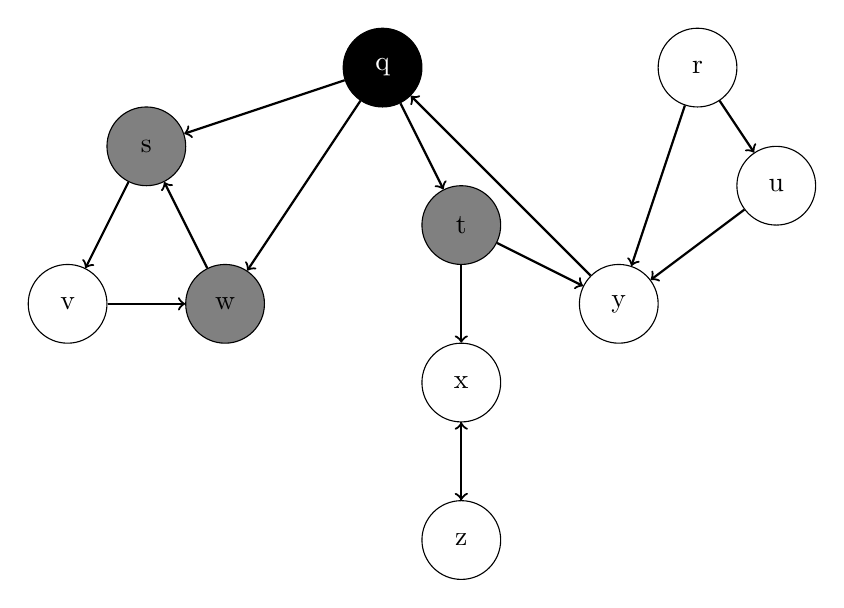
\begin{tikzpicture}[every node/.style={draw, circle, minimum size=1cm}]
              % Nodos
              \node (v) at (0,0) {v};
              \node[draw, circle, fill=gray] (s) at (1,2) {s};
              \node[draw, circle, fill=gray] (w) at (2,0) {w};
              \node[draw, circle, fill=black, text=white] (q) at (4,3) {q};
              \node[draw, circle, fill=gray] (t) at (5,1) {t};
              \node (y) at (7,0) {y};
              \node (r) at (8,3) {r};
              \node (u) at (9,1.5) {u};
              \node (x) at (5,-1) {x};
              \node (z) at (5,-3) {z};
              
              % Aristas
              \draw[->, thick] (s) -- (v);
              \draw[->, thick] (v) -- (w);
              \draw[->, thick] (w) -- (s);
              \draw[->, thick] (q) -- (s);
              \draw[->, thick] (q) -- (w);
              \draw[->, thick] (q) -- (t);
              \draw[->, thick] (t) -- (y);
              \draw[->, thick] (y) -- (q);
              \draw[->, thick] (r) -- (y);
              \draw[->, thick] (u) -- (y);
              \draw[->, thick] (r) -- (u);
              \draw[->, thick] (t) -- (x);
              \draw[->, thick] (x) -- (z);
              \draw[->, thick] (z) -- (x);
            \end{tikzpicture}
          \end{center}
          \[
            \scalebox{1.5}{$
              \begin{array}{|c|c|c|c|c|}
                  \hline
                  s & w & t \\ 
                  \hline
              \end{array}
            $}
          \]

          \item Passo 3: Removo o nó “s” da filha. 
          Em seguida, adiciono seus nós adjacentes à filha; 
          neste caso, os nós adjacentes são "v".
          \begin{center}
            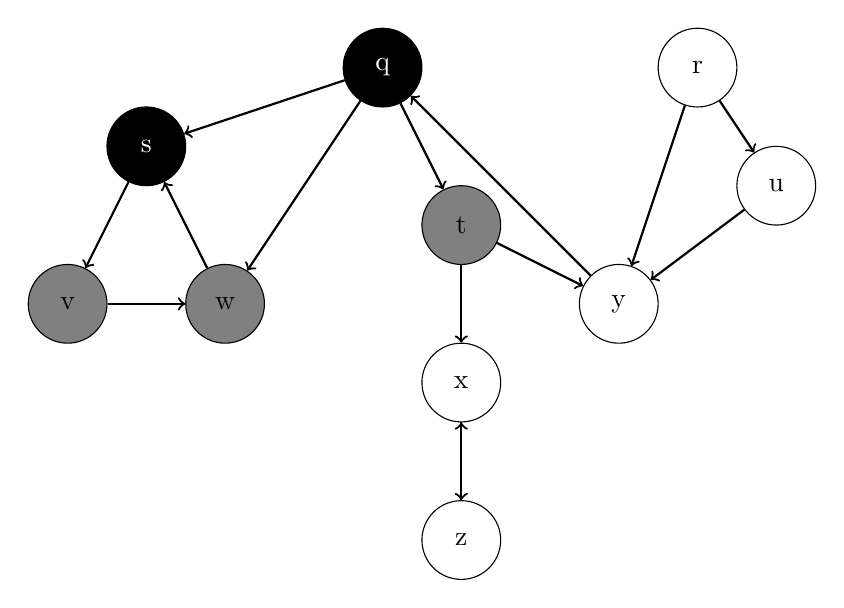
\begin{tikzpicture}[every node/.style={draw, circle, minimum size=1cm}]
              % Nodos
              \node[draw, circle, fill=gray] (v) at (0,0) {v};
              \node[draw, circle, fill=black, text=white] (s) at (1,2) {s};
              \node[draw, circle, fill=gray] (w) at (2,0) {w};
              \node[draw, circle, fill=black, text=white] (q) at (4,3) {q};
              \node[draw, circle, fill=gray] (t) at (5,1) {t};
              \node (y) at (7,0) {y};
              \node (r) at (8,3) {r};
              \node (u) at (9,1.5) {u};
              \node (x) at (5,-1) {x};
              \node (z) at (5,-3) {z};
              
              % Aristas
              \draw[->, thick] (s) -- (v);
              \draw[->, thick] (v) -- (w);
              \draw[->, thick] (w) -- (s);
              \draw[->, thick] (q) -- (s);
              \draw[->, thick] (q) -- (w);
              \draw[->, thick] (q) -- (t);
              \draw[->, thick] (t) -- (y);
              \draw[->, thick] (y) -- (q);
              \draw[->, thick] (r) -- (y);
              \draw[->, thick] (u) -- (y);
              \draw[->, thick] (r) -- (u);
              \draw[->, thick] (t) -- (x);
              \draw[->, thick] (x) -- (z);
              \draw[->, thick] (z) -- (x);
            \end{tikzpicture}
          \end{center}
          \[
            \scalebox{1.5}{$
              \begin{array}{|c|c|c|c|c|}
                  \hline
                  w & t & v \\ 
                  \hline
              \end{array}
            $}
          \]
        
          \item Passo 4: Removo o nó “w” da filha. 
          Em seguida, adiciono seus nós adjacentes à filha; 
          neste caso, já não tem nós adjacentes.
          \begin{center}
            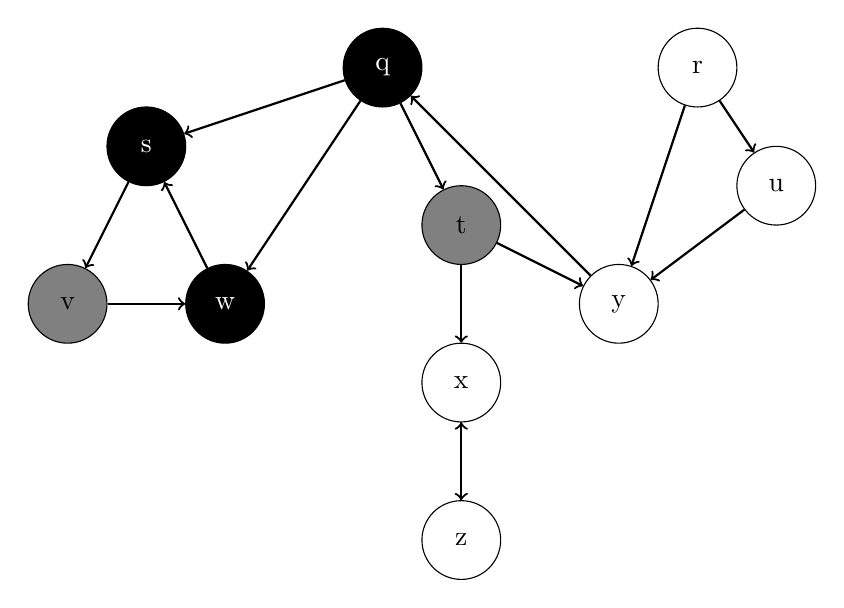
\begin{tikzpicture}[every node/.style={draw, circle, minimum size=1cm}]
              % Nodos
              \node[draw, circle, fill=gray] (v) at (0,0) {v};
              \node[draw, circle, fill=black, text=white] (s) at (1,2) {s};
              \node[draw, circle, fill=black, text=white] (w) at (2,0) {w};
              \node[draw, circle, fill=black, text=white] (q) at (4,3) {q};
              \node[draw, circle, fill=gray] (t) at (5,1) {t};
              \node (y) at (7,0) {y};
              \node (r) at (8,3) {r};
              \node (u) at (9,1.5) {u};
              \node (x) at (5,-1) {x};
              \node (z) at (5,-3) {z};
              
              % Aristas
              \draw[->, thick] (s) -- (v);
              \draw[->, thick] (v) -- (w);
              \draw[->, thick] (w) -- (s);
              \draw[->, thick] (q) -- (s);
              \draw[->, thick] (q) -- (w);
              \draw[->, thick] (q) -- (t);
              \draw[->, thick] (t) -- (y);
              \draw[->, thick] (y) -- (q);
              \draw[->, thick] (r) -- (y);
              \draw[->, thick] (u) -- (y);
              \draw[->, thick] (r) -- (u);
              \draw[->, thick] (t) -- (x);
              \draw[->, thick] (x) -- (z);
              \draw[->, thick] (z) -- (x);
            \end{tikzpicture}
          \end{center}
          \[
            \scalebox{1.5}{$
              \begin{array}{|c|c|c|c|c|}
                  \hline
                  t & v \\ 
                  \hline
              \end{array}
            $}
          \]

          \item Passo 5: Removo o nó “t” da filha. 
          Em seguida, adiciono seus nós adjacentes à filha; 
          neste caso, os nós adjacentes são "x" e "y".
          \begin{center}
            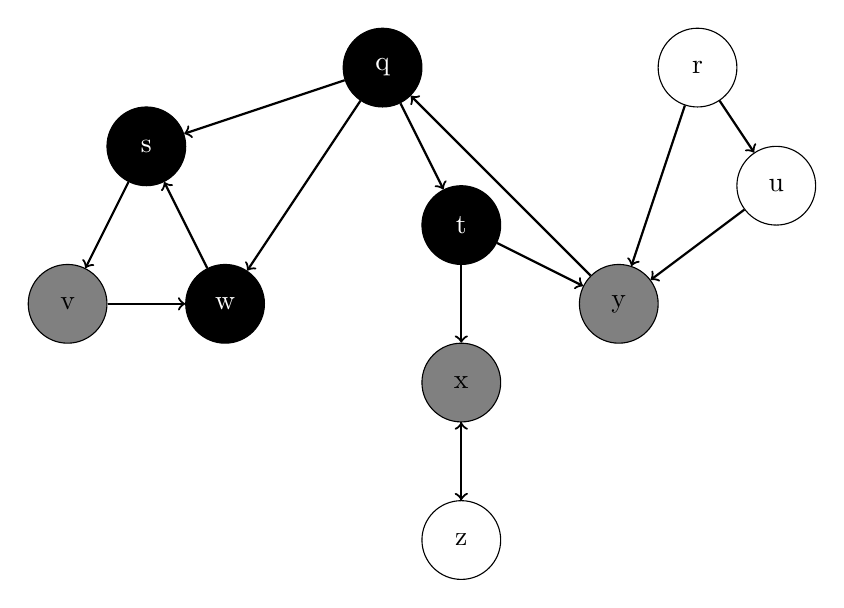
\begin{tikzpicture}[every node/.style={draw, circle, minimum size=1cm}]
              % Nodos
              \node[draw, circle, fill=gray] (v) at (0,0) {v};
              \node[draw, circle, fill=black, text=white] (s) at (1,2) {s};
              \node[draw, circle, fill=black, text=white] (w) at (2,0) {w};
              \node[draw, circle, fill=black, text=white] (q) at (4,3) {q};
              \node[draw, circle, fill=black, text=white] (t) at (5,1) {t};
              \node[draw, circle, fill=gray] (y) at (7,0) {y};
              \node (r) at (8,3) {r};
              \node (u) at (9,1.5) {u};
              \node[draw, circle, fill=gray] (x) at (5,-1) {x};
              \node (z) at (5,-3) {z};
              
              % Aristas
              \draw[->, thick] (s) -- (v);
              \draw[->, thick] (v) -- (w);
              \draw[->, thick] (w) -- (s);
              \draw[->, thick] (q) -- (s);
              \draw[->, thick] (q) -- (w);
              \draw[->, thick] (q) -- (t);
              \draw[->, thick] (t) -- (y);
              \draw[->, thick] (y) -- (q);
              \draw[->, thick] (r) -- (y);
              \draw[->, thick] (u) -- (y);
              \draw[->, thick] (r) -- (u);
              \draw[->, thick] (t) -- (x);
              \draw[->, thick] (x) -- (z);
              \draw[->, thick] (z) -- (x);
            \end{tikzpicture}
          \end{center}
          \[
            \scalebox{1.5}{$
              \begin{array}{|c|c|c|c|c|}
                  \hline
                  v & x & y \\ 
                  \hline
              \end{array}
            $}
          \]

          \item Passo 6: Removo o nó “v” da filha. 
          Em seguida, adiciono seus nós adjacentes à filha; 
          neste caso, já não tem nós adjacentes.
          \begin{center}
            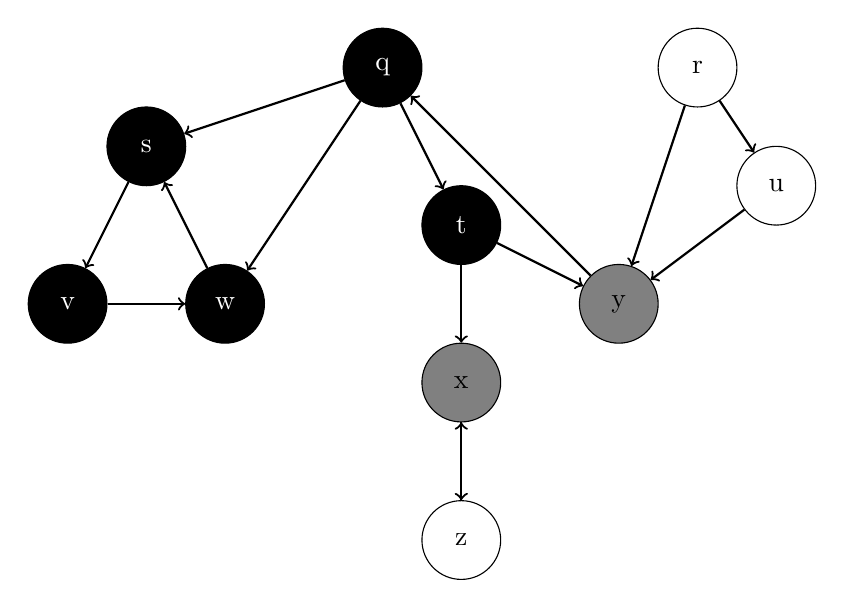
\begin{tikzpicture}[every node/.style={draw, circle, minimum size=1cm}]
              % Nodos
              \node[draw, circle, fill=black, text=white] (v) at (0,0) {v};
              \node[draw, circle, fill=black, text=white] (s) at (1,2) {s};
              \node[draw, circle, fill=black, text=white] (w) at (2,0) {w};
              \node[draw, circle, fill=black, text=white] (q) at (4,3) {q};
              \node[draw, circle, fill=black, text=white] (t) at (5,1) {t};
              \node[draw, circle, fill=gray] (y) at (7,0) {y};
              \node (r) at (8,3) {r};
              \node (u) at (9,1.5) {u};
              \node[draw, circle, fill=gray] (x) at (5,-1) {x};
              \node (z) at (5,-3) {z};
              
              % Aristas
              \draw[->, thick] (s) -- (v);
              \draw[->, thick] (v) -- (w);
              \draw[->, thick] (w) -- (s);
              \draw[->, thick] (q) -- (s);
              \draw[->, thick] (q) -- (w);
              \draw[->, thick] (q) -- (t);
              \draw[->, thick] (t) -- (y);
              \draw[->, thick] (y) -- (q);
              \draw[->, thick] (r) -- (y);
              \draw[->, thick] (u) -- (y);
              \draw[->, thick] (r) -- (u);
              \draw[->, thick] (t) -- (x);
              \draw[->, thick] (x) -- (z);
              \draw[->, thick] (z) -- (x);
            \end{tikzpicture}
          \end{center}
          \[
            \scalebox{1.5}{$
              \begin{array}{|c|c|c|c|c|}
                  \hline
                  x & y \\ 
                  \hline
              \end{array}
            $}
          \]

          \item Passo 7: Removo o nó “x” da filha. 
          Em seguida, adiciono seus nós adjacentes à filha; 
          neste caso, os nós adjacentes são "z".
          \begin{center}
            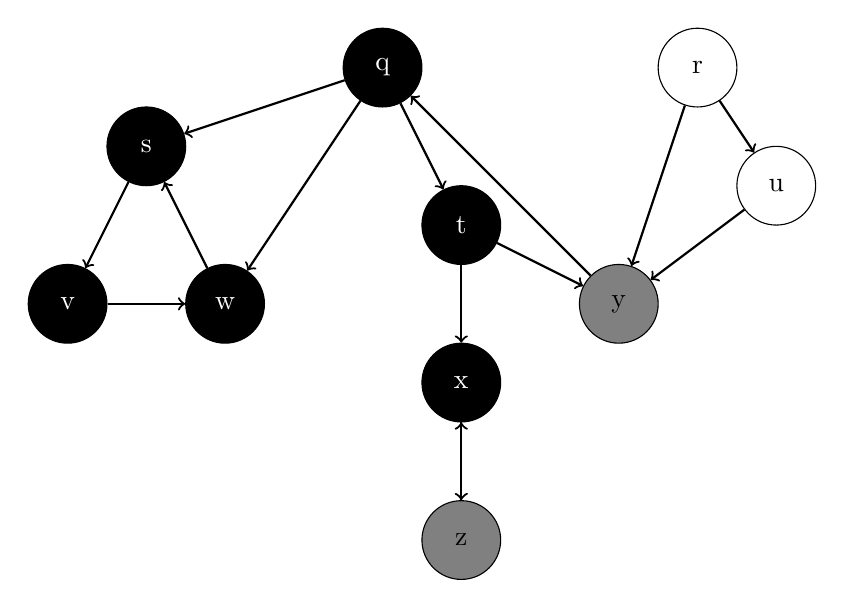
\begin{tikzpicture}[every node/.style={draw, circle, minimum size=1cm}]
              % Nodos
              \node[draw, circle, fill=black, text=white] (v) at (0,0) {v};
              \node[draw, circle, fill=black, text=white] (s) at (1,2) {s};
              \node[draw, circle, fill=black, text=white] (w) at (2,0) {w};
              \node[draw, circle, fill=black, text=white] (q) at (4,3) {q};
              \node[draw, circle, fill=black, text=white] (t) at (5,1) {t};
              \node[draw, circle, fill=gray] (y) at (7,0) {y};
              \node (r) at (8,3) {r};
              \node (u) at (9,1.5) {u};
              \node[draw, circle, fill=black, text=white] (x) at (5,-1) {x};
              \node[draw, circle, fill=gray] (z) at (5,-3) {z};
              
              % Aristas
              \draw[->, thick] (s) -- (v);
              \draw[->, thick] (v) -- (w);
              \draw[->, thick] (w) -- (s);
              \draw[->, thick] (q) -- (s);
              \draw[->, thick] (q) -- (w);
              \draw[->, thick] (q) -- (t);
              \draw[->, thick] (t) -- (y);
              \draw[->, thick] (y) -- (q);
              \draw[->, thick] (r) -- (y);
              \draw[->, thick] (u) -- (y);
              \draw[->, thick] (r) -- (u);
              \draw[->, thick] (t) -- (x);
              \draw[->, thick] (x) -- (z);
              \draw[->, thick] (z) -- (x);
            \end{tikzpicture}
          \end{center}
          \[
            \scalebox{1.5}{$
              \begin{array}{|c|c|c|c|c|}
                  \hline
                  y & z \\ 
                  \hline
              \end{array}
            $}
          \]

          \item Passo 8: Removo o nó “y” da filha. 
          Em seguida, adiciono seus nós adjacentes à filha; 
          neste caso, já não tem nós adjacentes.
          \begin{center}
            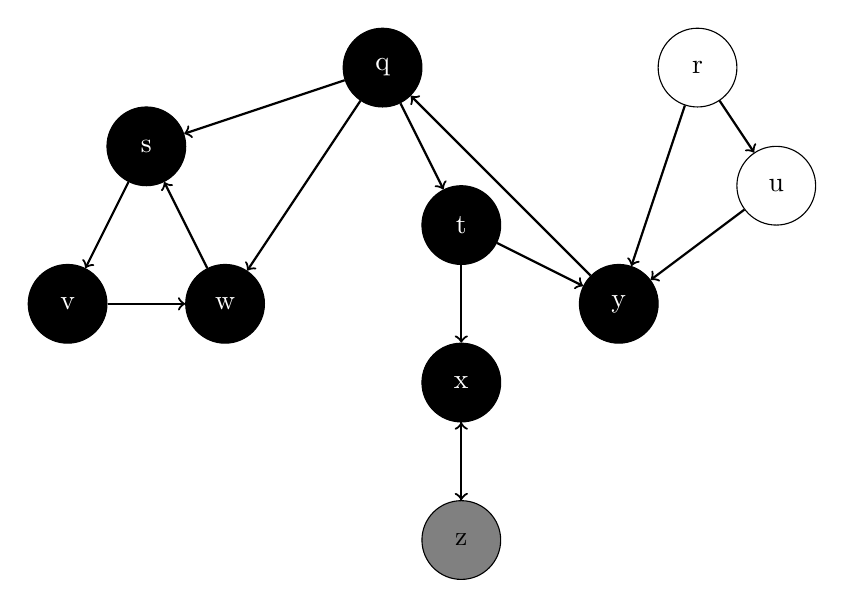
\begin{tikzpicture}[every node/.style={draw, circle, minimum size=1cm}]
              % Nodos
              \node[draw, circle, fill=black, text=white] (v) at (0,0) {v};
              \node[draw, circle, fill=black, text=white] (s) at (1,2) {s};
              \node[draw, circle, fill=black, text=white] (w) at (2,0) {w};
              \node[draw, circle, fill=black, text=white] (q) at (4,3) {q};
              \node[draw, circle, fill=black, text=white] (t) at (5,1) {t};
              \node[draw, circle, fill=black, text=white] (y) at (7,0) {y};
              \node (r) at (8,3) {r};
              \node (u) at (9,1.5) {u};
              \node[draw, circle, fill=black, text=white] (x) at (5,-1) {x};
              \node[draw, circle, fill=gray] (z) at (5,-3) {z};
              
              % Aristas
              \draw[->, thick] (s) -- (v);
              \draw[->, thick] (v) -- (w);
              \draw[->, thick] (w) -- (s);
              \draw[->, thick] (q) -- (s);
              \draw[->, thick] (q) -- (w);
              \draw[->, thick] (q) -- (t);
              \draw[->, thick] (t) -- (y);
              \draw[->, thick] (y) -- (q);
              \draw[->, thick] (r) -- (y);
              \draw[->, thick] (u) -- (y);
              \draw[->, thick] (r) -- (u);
              \draw[->, thick] (t) -- (x);
              \draw[->, thick] (x) -- (z);
              \draw[->, thick] (z) -- (x);
            \end{tikzpicture}
          \end{center}
          \[
            \scalebox{1.5}{$
              \begin{array}{|c|c|c|c|c|}
                  \hline
                  z \\ 
                  \hline
              \end{array}
            $}
          \]

          \item Passo 9: Removo o nó “z” da filha. 
          Em seguida, adiciono seus nós adjacentes à filha; 
          neste caso, já não tem nós adjacentes.
          \begin{center}
            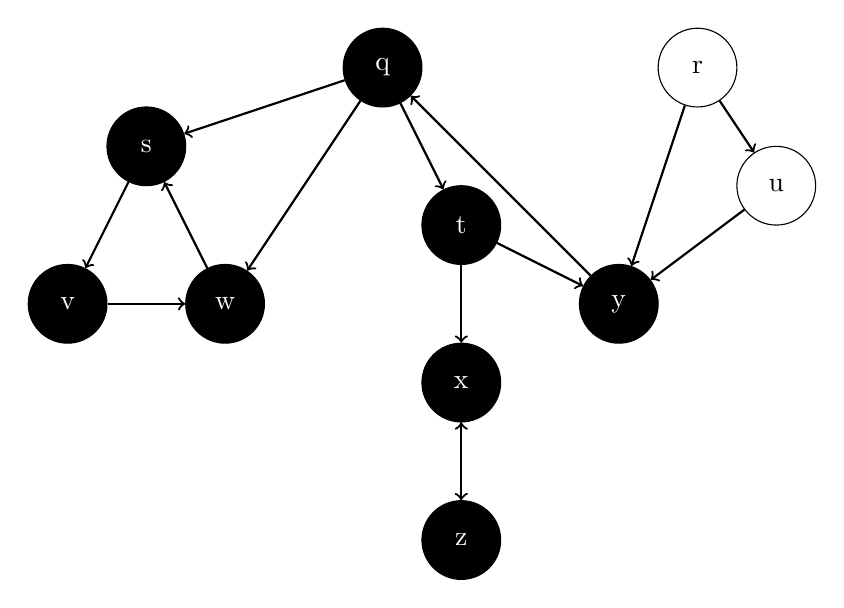
\begin{tikzpicture}[every node/.style={draw, circle, minimum size=1cm}]
              % Nodos
              \node[draw, circle, fill=black, text=white] (v) at (0,0) {v};
              \node[draw, circle, fill=black, text=white] (s) at (1,2) {s};
              \node[draw, circle, fill=black, text=white] (w) at (2,0) {w};
              \node[draw, circle, fill=black, text=white] (q) at (4,3) {q};
              \node[draw, circle, fill=black, text=white] (t) at (5,1) {t};
              \node[draw, circle, fill=black, text=white] (y) at (7,0) {y};
              \node (r) at (8,3) {r};
              \node (u) at (9,1.5) {u};
              \node[draw, circle, fill=black, text=white] (x) at (5,-1) {x};
              \node[draw, circle, fill=black, text=white] (z) at (5,-3) {z};
              
              % Aristas
              \draw[->, thick] (s) -- (v);
              \draw[->, thick] (v) -- (w);
              \draw[->, thick] (w) -- (s);
              \draw[->, thick] (q) -- (s);
              \draw[->, thick] (q) -- (w);
              \draw[->, thick] (q) -- (t);
              \draw[->, thick] (t) -- (y);
              \draw[->, thick] (y) -- (q);
              \draw[->, thick] (r) -- (y);
              \draw[->, thick] (u) -- (y);
              \draw[->, thick] (r) -- (u);
              \draw[->, thick] (t) -- (x);
              \draw[->, thick] (x) -- (z);
              \draw[->, thick] (z) -- (x);
            \end{tikzpicture}
          \end{center}
          \[
            \scalebox{1.5}{$
              \begin{array}{|c|c|c|c|c|}
                  \hline
                  \\ 
                  \hline
              \end{array}
            $}
          \]

      \end{enumerate}

    \item Indique quais vértices formam ciclo no grafo.
      \begin{enumerate}[label=\textbullet]
        \item Ciclo com 2 nós
          \begin{center}
            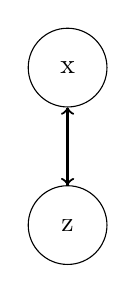
\begin{tikzpicture}[every node/.style={draw, circle, minimum size=1cm}]
              % Nodos
              \node(x) at (0,-1) {x};
              \node(z) at (0,-3) {z};
              
              % Aristas
              \draw[->, thick] (x) -- (z);
              \draw[->, thick] (z) -- (x);
            \end{tikzpicture}
          \end{center}
        \item Ciclo com 3 nós
        \begin{center}
          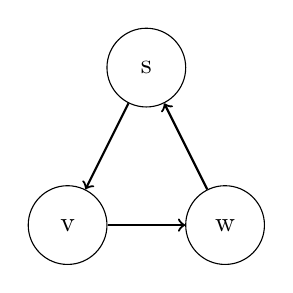
\begin{tikzpicture}[every node/.style={draw, circle, minimum size=1cm}]
            % Nodos
            \node (v) at (0,0) {v};
            \node (s) at (1,2) {s};
            \node (w) at (2,0) {w};
            
            % Aristas
            \draw[->, thick] (s) -- (v);
            \draw[->, thick] (v) -- (w);
            \draw[->, thick] (w) -- (s);
          \end{tikzpicture}
        \end{center}
      \end{enumerate}

      \begin{center}
        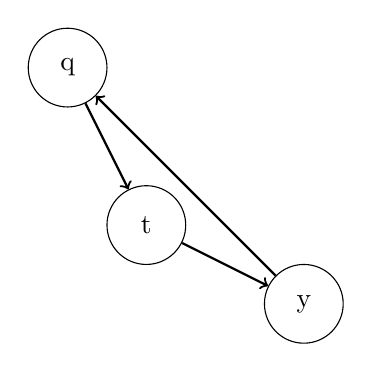
\begin{tikzpicture}[every node/.style={draw, circle, minimum size=1cm}]
          % Nodos
          \node(q) at (4,3) {q};
          \node(t) at (5,1) {t};
          \node(y) at (7,0) {y};
          
          % Aristas
          \draw[->, thick] (q) -- (t);
          \draw[->, thick] (t) -- (y);
          \draw[->, thick] (y) -- (q);
          
        \end{tikzpicture}
      \end{center}

    \item Tenho que remover as arestas de $"q"->"t"$, $"t" -> "y"$ e $"y" -> "q"$ para obter 3 componentes.
      \begin{center}
        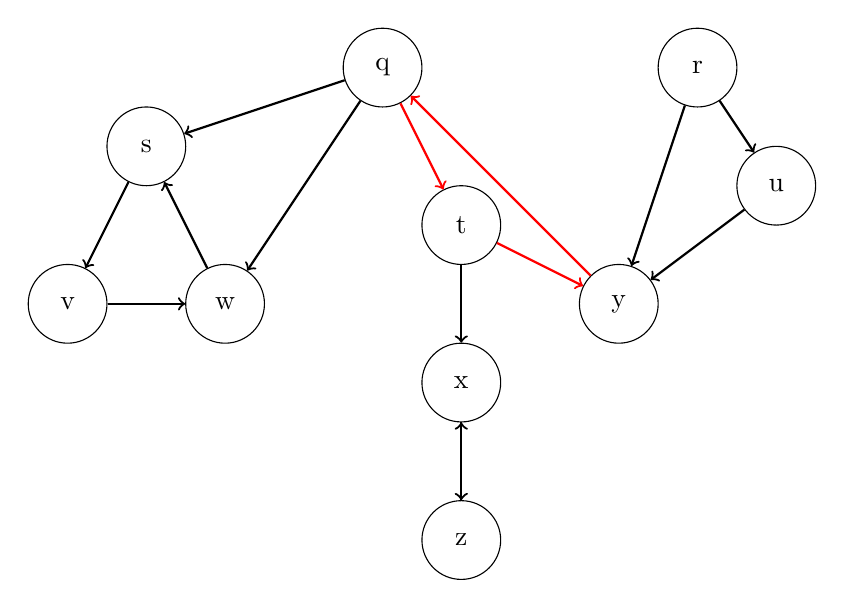
\begin{tikzpicture}[every node/.style={draw, circle, minimum size=1cm}]
          % Nodos
          \node(v) at (0,0) {v};
          \node(s) at (1,2) {s};
          \node(w) at (2,0) {w};
          \node(q) at (4,3) {q};
          \node(t) at (5,1) {t};
          \node(y) at (7,0) {y};
          \node (r) at (8,3) {r};
          \node (u) at (9,1.5) {u};
          \node(x) at (5,-1) {x};
          \node(z) at (5,-3) {z};
          
          % Aristas
          \draw[->, thick] (s) -- (v);
          \draw[->, thick] (v) -- (w);
          \draw[->, thick] (w) -- (s);
          \draw[->, thick] (q) -- (s);
          \draw[->, thick] (q) -- (w);
          \draw[->, thick, draw=red] (q) -- (t);
          \draw[->, thick, draw=red] (t) -- (y);
          \draw[->, thick, draw=red] (y) -- (q);
          \draw[->, thick] (r) -- (y);
          \draw[->, thick] (u) -- (y);
          \draw[->, thick] (r) -- (u);
          \draw[->, thick] (t) -- (x);
          \draw[->, thick] (x) -- (z);
          \draw[->, thick] (z) -- (x);
        \end{tikzpicture}
      \end{center}
  \end{enumerate}


  \subsection {(0.2) Quando usar BFS em vez de DFS?}
  \subsubsection{Solução:}
  Use BFS quando você precisar explorar um grafo em camadas, 
  ou seja, descobrir todos os vértices a uma certa distância antes 
  de prosseguir para os mais distantes. É útil para encontrar o 
  menor caminho em grafos não ponderados ou em problemas de 
  conectividade.

  \subsection {(0.2) BFS ou DFS seria mais indicado para encontrar 
  caminhos curtos em grafos não ponderados?}
  \subsubsection{Solução:}
  BFS é mais indicado, pois explora o grafo nível por nível e 
  garante que o primeiro caminho encontrado seja o mais curto em 
  grafos não ponderados.

  \subsection {(0.2) BFS ou DFS seria mais indicado para detectar 
  ciclos em grafos?}
  \subsubsection{Solução:}
  DFS é mais indicado para detectar ciclos, especialmente em 
  grafos direcionados, pois permite rastrear os ancestrais no 
  caminho atual de exploração, facilitando a identificação de 
  ciclos.
\end{document}